%&tex

\chapter{Pre-processing}\label{chp:preprocessing}

Before training and inference, we apply different image transformations to the dataset. As
mentioned in~\autoref{chp:modelling}, we use three main transformations: binarization, quantization
and equalization. In all cases we first convert the original RGB colored dataset to grayscale.

\section{Binarization}

The binarization process was done by first converting the original dataset to grayscale, followed
by applying a gaussian blur filter with a $(1, 1)$ kernel and $(1, 1)$ standard deviation, and
finally using Otsu's binarization. We chose this particular process since standard hard threshold
binarization was unable to produce clear images of the track lines.

\begin{figure}[h]
  \centering
  
\includegraphics[scale=1.75]{imgs/binary_left_h.png}
  
\includegraphics[scale=1.75]{imgs/binary_up_h.png}
  
\includegraphics[scale=1.75]{imgs/binary_right_h.png}
  \caption{Binarization using hard threshold.\label{fig:bin-hard}}
\end{figure}

\autoref{fig:bin-hard} shows how hard thresholding can produce noisy images, as the applied
threshold does not account for local neighborhoods and may end up choosing a bad threshold value.
\autoref{fig:bin-otsu} shows a sample of the dataset after applying Otsu's binarization, with much
clearer tracks. Images are labeled as left, up and right respectively

\begin{figure}[h]
  \centering
  
\includegraphics[scale=1.75]{imgs/binary_left.png}
  
\includegraphics[scale=1.75]{imgs/binary_up.png}
  
\includegraphics[scale=1.75]{imgs/binary_right.png}
  \caption{Binarization using Otsu's threshold.\label{fig:bin-otsu}}
\end{figure}

\section{Quantization}

The Gens-Domingos algorithm, as mentioned in~\autoref{chp:structure}, has two main steps: a
clustering phase and an independency test part. Our independency test implementation uses the
standard G-test statistical test based on contingency tables, where each frequency of the
categories of each two variables are laid out on a matrix and their likelihood ratios are computed.
This test takes only $\bigo(n m)$, where $n$ and $m$ are the number of categories of each variable.
However, each variable must be tested pairwise with all others, and although we use a spanning-tree
heuristic, time complexity grows fast the more categories and total number of variables there are.

We empirically found that $\max\{n,m\}$ and training set size are directly correlated to the
model's accuracy and speed. If $n$ or $m$ are big and the training set size is small, then accuracy
will fall. Accuracy increases if the training set is large, but is still dependent on how big the
number of categories in variables is. Our best results were with small $n$ and $m$ with a large
training set. Another interesting result we found is that the bigger the number of categories, the
shallower the SPN when using the Gens-Domingos algorithm, which results in much faster inference.

\begin{figure}[h]
  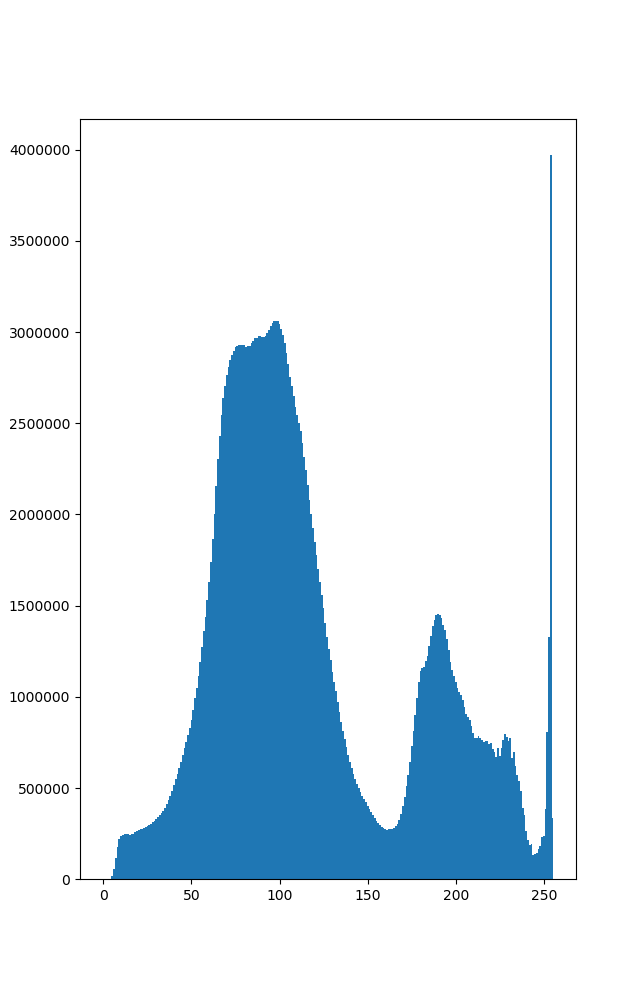
\includegraphics[scale=0.3]{imgs/hist_8.png}
  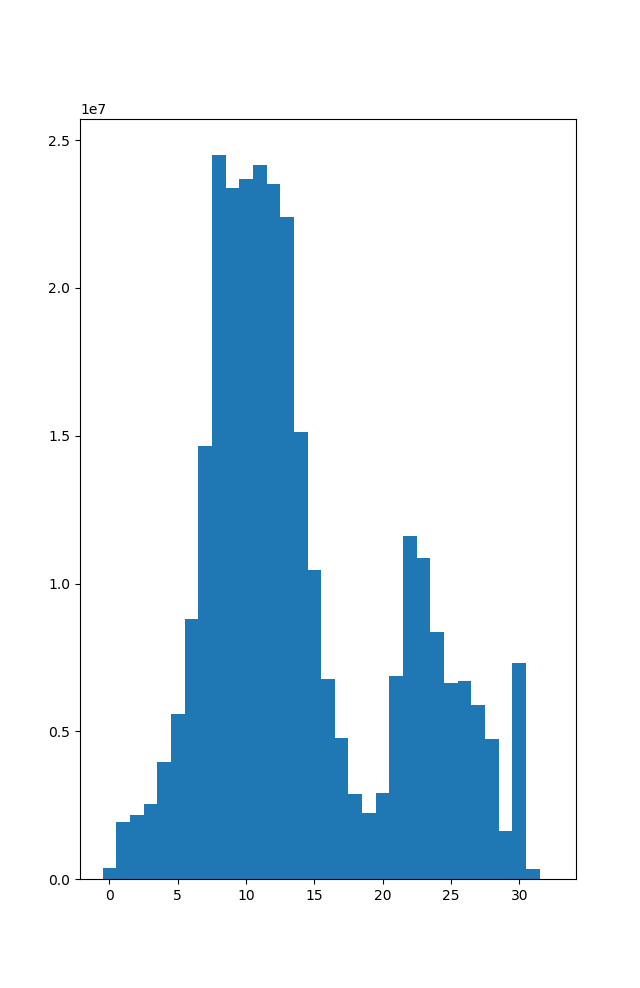
\includegraphics[scale=0.3]{imgs/hist_5.png}
  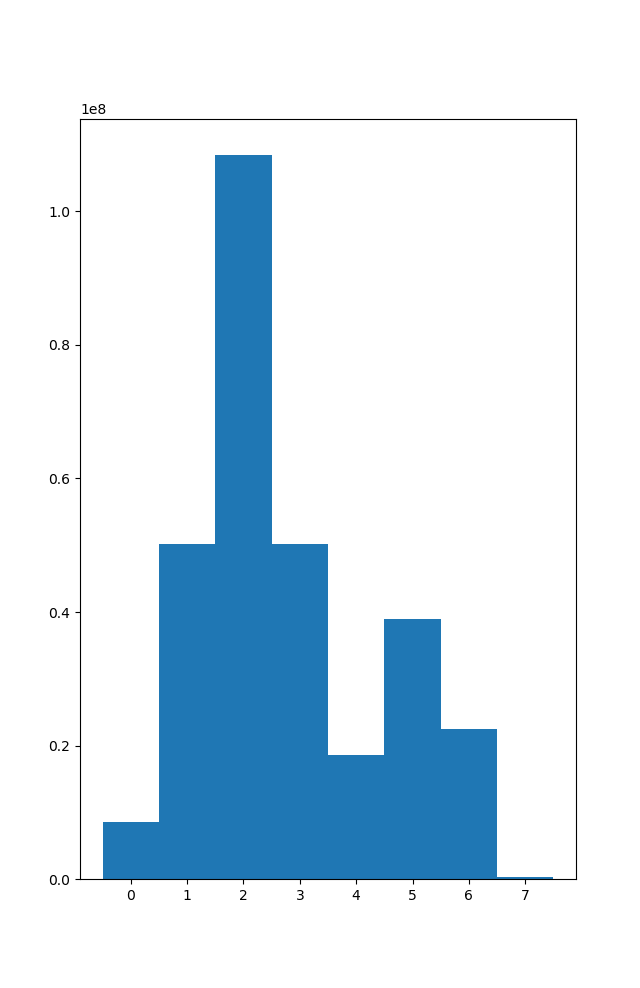
\includegraphics[scale=0.3]{imgs/hist_3.png}
  \caption{Histogram for dataset pixel values on 8-bit, 5-bit and 3-bit image
    resolutions.\label{fig:hist-orig}}
\end{figure}

A possible explanation for poor results with small training sets is the low number of pixel
intensity values for too extreme values, as there are fewer samples where pixels are either too
bright or too dark, as~\autoref{fig:hist-orig} shows. This is a problem for the G-test, as
chi-squared tests are unreliable when dealing with low frequencies.

Quantizing the dataset resulted in a significant improvement in accuracy to the model when training
with a small set of images ($\leq$ 300). We found that when we increased the number of training
images, accuracy depended less on quantization, but inference time increased, as the model grew in
depth. We thus needed to find a balance between network complexity and accuracy.

We faced two possible solutions to this problem. Either implement an exact independence test, such
as the Fisher exact test (\cite{fisher-exact}), or perform histogram equalization on the dataset.
The former was unfortunately not an option, as we found that there were no libraries in Go or C
that provided a general case implementation of the Fisher exact test, and implementing our own
within our time constraints was out of question. We chose the latter, applying histogram
equalization on the entire dataset.

\section{Equalization}

Equalization was done using OpenCV. We attempted two methods of histogram equalization: traditional
equalization through brightness and contrast normalization, and Contrast Limited Adaptive Histogram
Equalization (CLAHE) (\cite{clahe}). We found that the CLAHE method resulted in images that were
very similar to the output of the traditional method. Since these transformations are also expected
to be applied on-the-fly during inference, we chose the standard equalization for its speed.
\autoref{fig:hist-eq} shows how the dataset pixel histogram looks like after equalization.

\begin{figure}[h]
  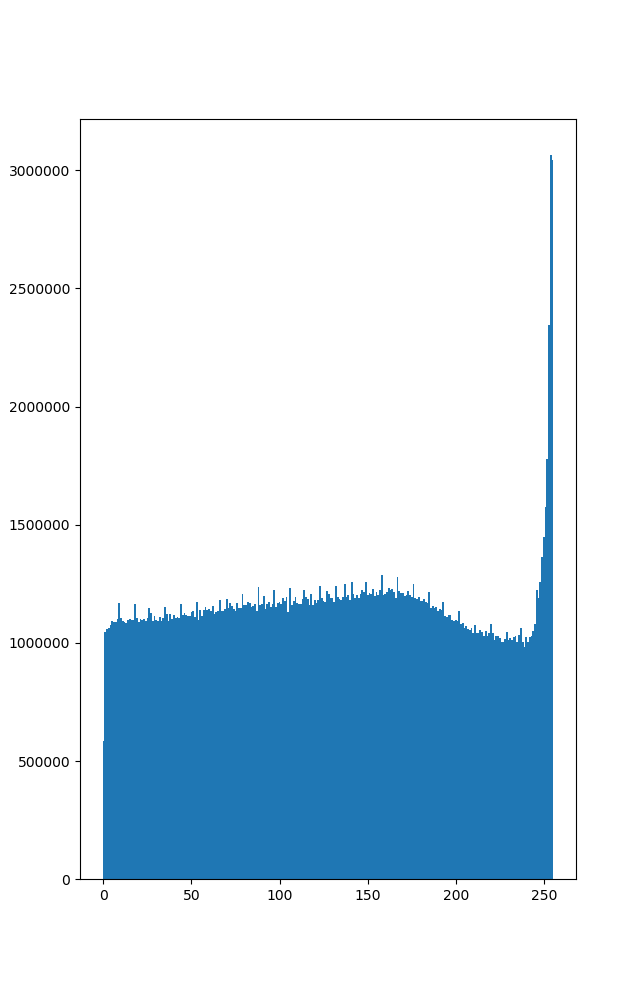
\includegraphics[scale=0.3]{imgs/hist_8_eq.png}
  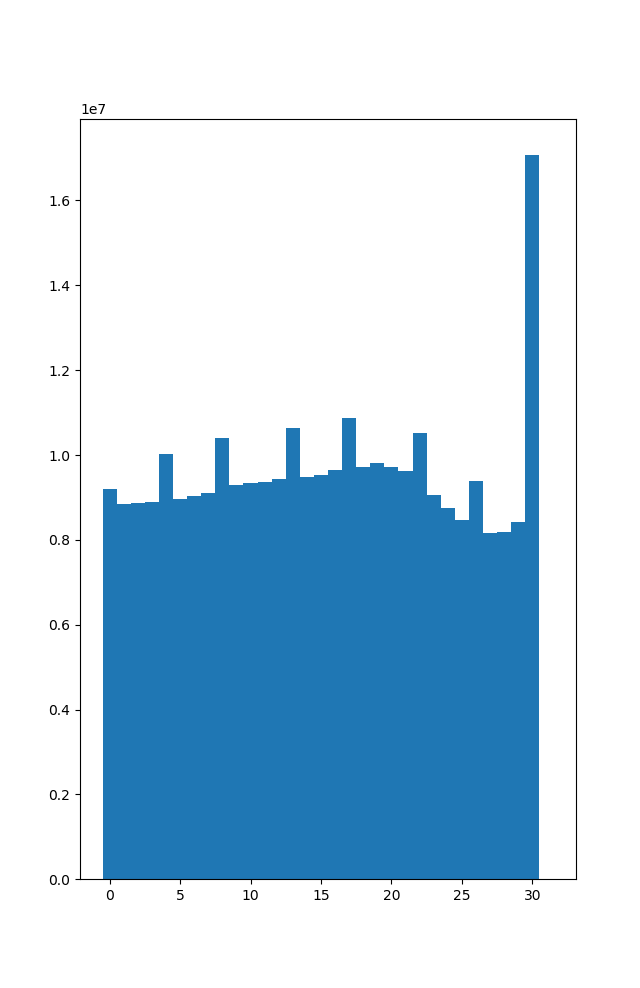
\includegraphics[scale=0.3]{imgs/hist_5_eq.png}
  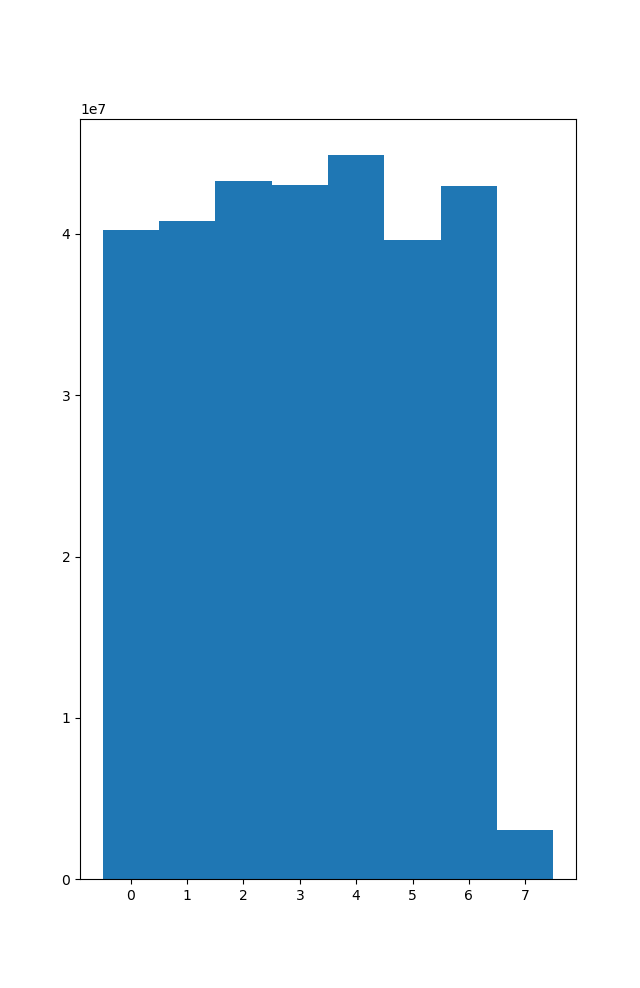
\includegraphics[scale=0.3]{imgs/hist_3_eq.png}
  \caption{Histogram for equalized dataset with 8-bit, 5-bit and 3-bit image
  resolutions.\label{fig:hist-eq}}
\end{figure}

When coupling quantization and equalization, we slightly increased accuracy, reaching up to a
$\approx$4\% accuracy difference.  Interestingly, these transformations proved to be harmful for
the Dennis-Ventura architecture. In fact, the structure yielded better results without
equalization, and quantization had little to no impact on accuracy. We attribute this phenomenom to
the classification architecture we discussed in~\autoref{chp:structure}. Since each sub-SPN is
essentially modelling each class as a separate, independent image model to the other classes, the
more details in the image, the easier the model can distinguish from other label images.
Furthermore, since the Dennis-Ventura algorithm does not need to run an independence test, it does
not suffer from its drawbacks and thus does not depend on an equalized histogram.
